\documentclass[a4paper,12pt]{article} % тип документа

% Поля страниц
\usepackage[left=2.5cm,right=2.5cm,
    top=2cm,bottom=2cm,bindingoffset=0cm]{geometry}
    
%Пакет дял таблиц   
\usepackage{multirow} 
    
%Отступ после заголовка    
\usepackage{indentfirst}


% Рисунки
\usepackage{floatrow,graphicx,calc}
\usepackage{wrapfig}

%%% Работа с картинками
\usepackage{graphicx}  % Для вставки рисунков
\graphicspath{{images/}{images2/}}  % папки с картинками
\setlength\fboxsep{3pt} % Отступ рамки \fbox{} от рисунка
\setlength\fboxrule{1pt} % Толщина линий рамки \fbox{}
\usepackage{wrapfig} % Обтекание рисунков и таблиц текстом

% Создаёем новый разделитель
\DeclareFloatSeparators{mysep}{\hspace{1cm}}

% Ссылки?
\usepackage{hyperref}
\usepackage[rgb]{xcolor}
\hypersetup{				% Гиперссылки
    colorlinks=true,       	% false: ссылки в рамках
	urlcolor=blue          % на URL
}


%  Русский язык
\usepackage[T2A]{fontenc}			% кодировка
\usepackage[utf8]{inputenc}			% кодировка исходного текста
\usepackage[english,russian]{babel}	% локализация и переносы




% Математика
\usepackage{amsmath,amsfonts,amssymb,amsthm,mathtools}

%%% Дополнительная работа с математикой
\usepackage{amsmath,amsfonts,amssymb,amsthm,mathtools} % AMS
\usepackage{icomma} % "Умная" запятая: $0,2$ --- число, $0, 2$ --- перечисление


% Что-то 
\usepackage{wasysym}


\begin{document}
\begin{center}
	\footnotesize{МОСКОВСКИЙ ФИЗИКО-ТЕХНИЧЕСКИЙ ИНСТИТУТ\\(НАЦИОНАЛЬНЫЙ 			ИССЛЕДОВАТЕЛЬСКИЙ УНИВЕРСИТЕТ)}\\
	\footnotesize{ФИЗТЕХ-ШКОЛА РАДИОТЕХНИКИ И КОМПЬЮТЕРНЫХ ТЕХНОЛОГИЙ\\}
	\hfill \break
	\hfill \break
	\hfill \break
	\hfill \break
	\hfill \break
	\hfill \break
\end{center}

\begin{center}   
    \hfill \break
	\hfill \break
	\hfill \break
	\hfill \break
	\hfill \break
	\hfill \break
	\hfill \break
	\hfill \break
	\hfill \break
	\hfill \break
	\hfill \break
	\large{Лабораторная работа № 3.2.1\\\large{\textbf{Сдвиг фаз в цепи переменного тока}}}\\
	\hfill \break
	\hfill \break
	\hfill \break
	\hfill \break
	\hfill \break
	\hfill \break
	\hfill \break
	\hfill \break
	\hfill \break
	\hfill \break
	\hfill \break
	\begin{flushright}
		Климова Екатерина\\
		Группа Б01-108
	\end{flushright}
	\hfill \break
\end{center}
\hfill \break
\hfill \break
\begin{center}
	Долгопрудный, 2022 г.
\end{center}
\thispagestyle{empty}

\newpage
\hfill \break
\textbf{Цель работы:} изучить влияние активного сопротивления, индуктивности и емкости на сдвиг фаз между током и напряжением в цепи переменного тока.
\hfill \break
\hfill \break
\textbf{В работе используются:} генератор звуковой частоты (ЗГ); двухканальный осциллограф (ЭО); магазин емкостей; магазин сопротивлений; катушка индуктивности; резисторы; универсальный измеритель импеданса ($LCR$-метр).

\section{Аннотация}
\hfill \break В работе предлагается исследовать зависимость сдвига фаз между током и напряжением от сопротивления в $RC$- и $RLC$-цепи; определить добротности колебательного контура, сняв зависимость сдвига фаз от частоты вблизи резонанса; оценить диапазон работы фазовращателя.

\section{Теоретические сведения}
\subsection{Вынужденные колебания}
\hfill \break Рассмотрим процессы, протекающие в $RLC$-контуре, подключенном к источнику внешней ЭДС, изменяющейся по гармоническому закону $\varepsilon = \varepsilon_{0}\cos{\omega t + \varphi_{0}}$. Тогда для напряжения в конденсаторе получим уравнение:

\begin{equation}\label{ linkname }
\ddot{U_{c}} + 2\gamma \dot{U_{c}} + \omega_{0}^2U_{c} = \omega_{0}^2\varepsilon_{0}\cos{\omega t + \varphi_{0}},
\end{equation}

\begin{wrapfigure}{l}{0.2\textwidth}
\begin{center}
    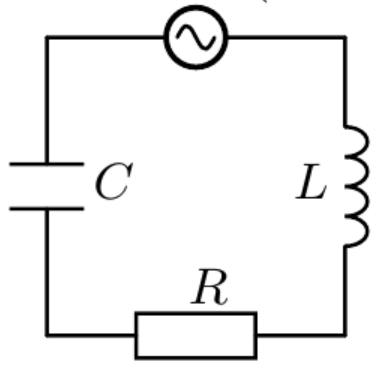
\includegraphics[width=1\textwidth]{3.2.1_1.png}
    \textbf{Рис. 1.} Последовательный контур с внешней ЭДС
\end{center}
\end{wrapfigure}

\hfill \break решение которого будет состоять из общего решения однородного дифференциального уравнения и какого-либо частного решения данного уравнения с правой частью. Для нахождения этого частного решения воспользуемся \textbf{методом комплексных амплитуд}. То есть \textit{пусть некоторая комплексная функция $f(t)$ является решением линейного дифференциального уравнения с вещественными коэффициентами и комплексной правой частью; тогда вещественная часть этой функции $Re f(t)$ является решением того же уравнения, в правой части которого стоит вещественная часть прежнего выражения, а мнимая часть $Im f(t)$ $-$ решением уравнения с мнимой правой частью.} Тогда уравнение (1) станет выглядеть так:

\begin{equation}\label{ linkname }
\ddot{U_{c}} + 2\gamma \dot{U_{c}} + \omega_{0}^2U_{c} = \omega_{0}^2\varepsilon,
\end{equation}

\hfill \break где $\varepsilon_{0}e^{i\varphi}$ называется \textbf{комплексной амплитудой}. Определим величину $Z$ $-$ \textbf{импеданс}, или комплексное сопротивление, $-$ характеристику колебательного контура на заданной частоте:

$$
Z_{R} = R, \text{ } Z_{L} = i\omega L, \text{ } Z_{C} =  \frac{1}{i\omega C}.
$$

\hfill \break Активным сопротивлением называется действительная часть $Z$, реактивным $-$ мнимая: $Im Z = \omega L - \frac{1}{\omega C}$. Импедансы контура и его отдельных элементов могут быть представлены в показательной форме:

\begin{equation}\label{ linkname }
Z = Z_{0}e^{i\psi},
\end{equation}

\hfill \break где $Z_{0}$ $-$ модуль комплексного числа, $\psi = arg Z$ $-$ его аргумент. Для импеданса рассматриваемого последовательного контура находим:

\begin{equation}\label{ linkname }
Z_{0} = \sqrt{(Re Z)^2 + (Im Z)^2} = \frac{R}{\cos{\psi_{I}}},
\end{equation}

\begin{equation}\label{ linkname }
\tg{\psi_{I}} = \frac{Im Z}{Re Z} = \frac{\omega L - \frac{1}{\omega C}}{R}.
\end{equation}

\hfill \break Так, действительная часть тока в контуре:

\begin{equation}\label{ linkname }
I(t) = \frac{\varepsilon_{0}}{R} \cos{\psi_{I}} \cos({\omega t + \varphi_{0} - \psi_{I}}).
\end{equation}

\hfill \break Как видно из (6), угол $\psi_{I}$, определяемый отношением мнимой и действительной частей импеданса, представляет собой сдвиг фаз между напряжением на последовательном контуре и током в нем, причем положительные значения этого угла соответствуют отставанию фазы тока, а отрицательные $-$ опережению. В общем случае, когда к источнику последовательно подключены резистор, конденсатор и катушка, сдвиг фазы тока лежит в пределах $-\pi/2 < \psi_{I} < \pi/2$. От этого угла также зависит амплитуда силы тока.

\subsection{Векторные диаграммы}
\hfill \break Решения, полученные методом комплексных амплитуд, допускают простую геометрическую интерпретацию. Комплексное число, например, напряжение $\varepsilon =\varepsilon_{0}e^{i(\omega t + \varphi_{0})}$, представляется на комплексной плоскости вектором, длина которого равна $\varepsilon_{0}$, а угол, составляемый этим вектором с  вещественной осью, равен $(\omega t + \varphi_{0})$ $-$ фазе напряжения. Вектор напряжения вращается со скоростью $\omega$ против часовой стрелки. Удобно перейти к системе координат, которая сама вращается с такой угловой скоростью. В этой системе вектор $\varepsilon$ будет представлен покоящимся вектором $\varepsilon_{0}e^{i \varphi}$, а векторы $\textbf{I}_{0}$, $\textbf{U}_{C0}$, $\textbf{U}_{L0}$, $\textbf{U}_{R0}$ тоже будут неподвижны, но окажутся сдвинутыми по углу относительно вектора $\varphi_{0}$. Вектор $\textbf{I}_{0}$, как показано выше, сдвинут от вектора $\varphi_{0}$ на угол $\psi_{I}$. Построенная таким образом диаграмма называется \textit{векторной}.

\subsection{Нахождение фазового сдвига}
\hfill \break Можно предложить два способа измерения разности фаз.

\hfill \break В \textit{первом способе} два сигнала $U_{1}$ и $U_{2}$ подаются на горизонтальную (канал $X$) и вертикальную (канал $Y$) развертки осциллографа. Смещение луча по горизонтали и вертикали определяется выражениями

$$
x = x_{0}\cos{\omega t}, \text{ } y = y_{0} \cos{(\omega t + \psi),}
$$

\hfill \break где $\psi$ $-$ сдвиг фаз между напряжениями $U_{1}$ и $U_{2}$, а $x_{0}$ и $y_{0}$ $-$ амплитуда напряжений, умноженные на коэффиенты усиления соответствующих каналов осциллографа. Исключив время, найдем, что

$$
\left(\frac{x}{x_{0}}\right)^2 + \left(\frac{y}{y_{0}}\right)^2 + \frac{2xy}{x_{0}y_{0}}\cos{\psi} = \sin^2{\psi}.
$$

\begin{wrapfigure}{r}{0.3\textwidth}
\begin{center}
    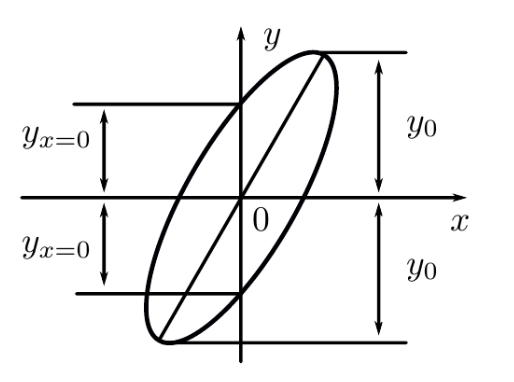
\includegraphics[width=1\textwidth]{3.2.1_2.png}
    \textbf{Рис. 2.} Эллипс на экране осциллографа
\end{center}
\end{wrapfigure}

\hfill \break Полученное выражение определяет эллипс, описываемый электронным лучом на экране осциллографа (рис. 2). Ориентация эллипса зависит как от искомого угла $\psi$, так и от усиления каналов осциллографа. Для расчета сдвига фаз можно измерить отрезки $2y_{x=0}$ и $2y_{0}$ и, подставляя эти значения в уравнение эллипса, найти

\begin{equation}\label{ linkname }
\psi = \pm \arcsin{\left( \frac{y_{x=0}}{y_{0}} \right)}.
\end{equation}

\hfill \break Для правильного измерения отрезка $2y_{x=0}$ важно, чтобы центр эллипса лежал на оси $y$.

\hfill \break \textit{Второй способ} заключается в непосредственном измерении сдвига фаз между сигналами на экране двухканального осциллографа. Напряжения $U_{1}$ и $U_{2}$ одновременно подаются на входные каналы ЭО при включенной внутренней горизонтальной развертке. При этом сигналы одновременно отображаются на экране. Измерение разности фаз в таком случае удобно проводить следующим образом:

\begin{enumerate}
\item подобрать частоту горизонтальной развертки, при которой на экране укладывается чуть больше половины периода синусоиды;
\item отцентрировать горизонтальную ось;
\item измерить расстояние $x_{0}$ между нулевыми значениями одного из сигналов, что соответствует разности фаз $\pi$;
\item измерить расстояние $x$ между нулевыми значениями двух синусоид и пересчитать сдвиг по фазе: $\psi = \pi x/x_{0}$. На рис. 3 синусоиды на экране ЭО сдвинуты по фазе на $\pi/2$.
\end{enumerate}

\section{Экспериментальная установка}
\hfill \break Схема установки для исследования сдвига фаз между током и напряжением в цепи переменного тока представлена на рис. 3. Эталонная катушка $L$, магазин емкостей $C$ и магазин сопротивлений $R$ соединены последовательно и через дополнительное сопротивление $r$ подключены к источнику синусоидального напряжения $-$ звуковому генератору (ЗГ).

\begin{center}
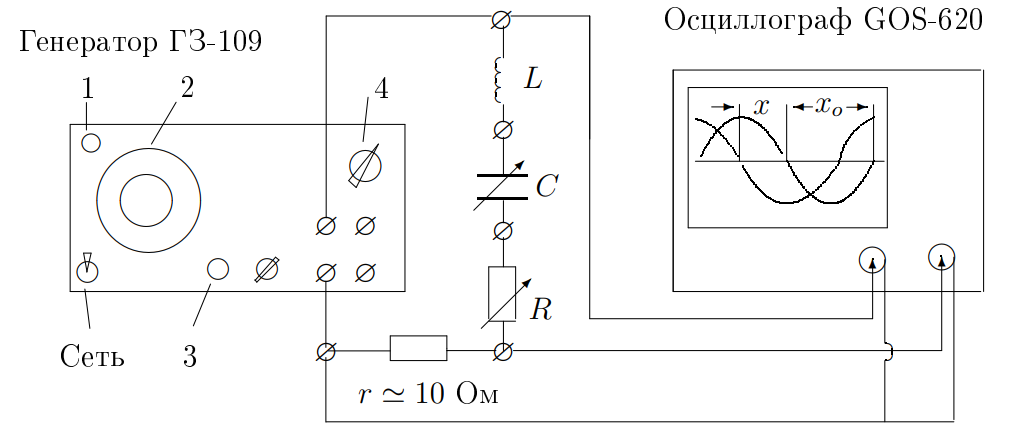
\includegraphics[width=0.85\linewidth]{3.2.1_3.png}\\
\textbf{Рис. 3.} Схема установки для исследования сдвига фаз между током и напряжением\\
\end{center}

\hfill \break Сигнал, пропорциональный току, снимается с сопротивления $r$, пропорциональный напряжению, $-$ с генератора. Оба сигнала подаются на ЭО, имеющий два канала вертикального отклонения. Измерение разности фаз можно проводить одним из двух описанных выше способов.

\hfill \break На практике часто используются устройства, называемые \textit{фазовращателями} ($0 < \psi < \pi)$. Схема фазовращателя, применяемого в данной работе, изображена на рис. 4. Она содержит два одинаковых резистора $R_{1}$, смонтированных на отдельной плате, магазин сопротивлений $R$ и магазин емкостей $C$.

\begin{center}
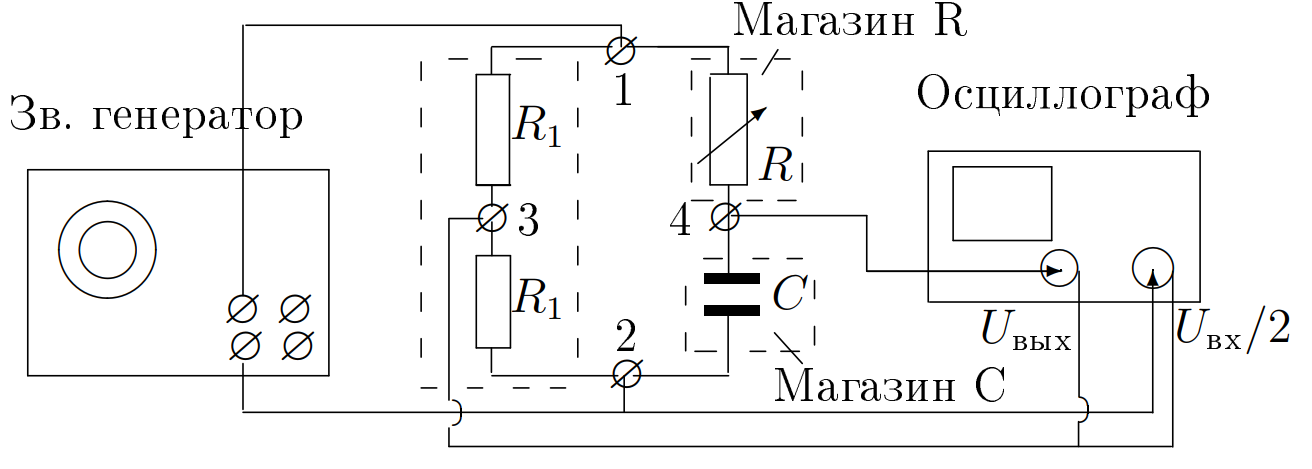
\includegraphics[width=0.85\linewidth]{3.2.1_4.png}\\
\textbf{Рис. 4.} Схема установки для исследования фазовращателя\\
\end{center}

\hfill \break Найдем, как зависит сдвиг фаз между входным напряжением $U_\text{вх} = U_{0}\cos{\omega t}$ (точки 1 и 2 на рис. 4) и выходным напряжением $U_\text{вых}$ (точки 3 и 4) от соотношения между импедансами сопротивления $R$ и емкости $C$. Для соответствующих комплексных амплитуд имеет место соотношение:

\begin{equation}\label{ linkname }
U_\text{вых} = \frac{U_\text{вх}}{2} \frac{R+\frac{i}{\omega C}}{R-\frac{i}{\omega C}}.
\end{equation}

\hfill \break Числитель и знаменатель (8) $-$ комплексно-сопряженные величины, модули которых одинаковы. Поэтому амплитуда выходного напряжения не зависит от $R$ и всегда равна $U_{0}/2$. Сдвиг фаз между выходным и входным напряжениями равен

\begin{equation}\label{ linkname }
\psi = \arg{\frac{U_\text{вых}}{U_\text{вх}}} = 2\arctg{\frac{1}{\omega RC}}.
\end{equation}

\hfill \break Он может меняться от $\psi = \pi$ при $R \rightarrow 0$ до $\psi = 0$ при $R \rightarrow \infty$.

\section{Ход работы}
\subsection{Исследование сдвига фаз в $RC$-цепи}
\hfill \break Для начала соберем схему, изображенную на рис. 3, и занесем в таблицу 1 некоторые параметры установки:

\begin{center}
\begin{tabular}{|c|c|}\hline
$ r $, Ом & $ R_{L} $, Ом\\\hline
$ 12.2 $ & $ 31.5 $\\\hline
\end{tabular} \\
\hfill \break \textbf {Таблица 1.} Некоторые параметры установки \\
\end{center}
 
\hfill \break Здесь $r$ $-$ дополнительное сопротивление, $R_{L}$ $-$ сопротивление катушки. Установим рабочую частоту $\nu = 1$ кГц, закоротим катушку (так как хотим исследовать $RC$-цепь), подключив оба провода, идущих к ней, к одной клемме, и установим на магазине емкостей $C = 0.5$ мкФ. Тогда реактивное сопротивление цепи: $X_{1} = 1/(\omega C) = 1/(2\pi \nu C) \approx 318$ Ом. Меняя сопротивление $R$ от $0$ до $10X_{1}$, измерим сдвиг фаз $\psi$ для каждого значения $R$. Результаты измерений занесем в таблицу 2:

\begin{center}
\begin{tabular}{|c|c|c|c|c|c|}\hline
$ R $, Ом & $ x $, дел & $ x_{0} $, дел & $ \psi $, рад & $ \omega CR_{\Sigma} $ & $ ctg(\psi) $\\\hline
0 & 8.00 & 17.00 & 1.48 & 0.04 & 0.09 \\\hline
159 & 6.50 & 18.50 & 1.10 & 0.54 & 0.50 \\\hline
318 & 4.50 & 17.50 & 0.81 & 1.04 & 0.96 \\\hline
636 & 3.00 & 20.00 & 0.47 & 2.04 & 1.96 \\\hline
954 & 2.00 & 20.00 & 0.31 & 3.04 & 3.08 \\\hline
1272 & 1.50 & 20.00 & 0.24 & 4.03 & 4.17 \\\hline
1908 & 1.00 & 20.00 & 0.16 & 6.03 & 6.31 \\\hline
\end{tabular} \\
\hfill \break \textbf {Таблица 2.} Расчеты и измерения для определения разности фаз в $RC$-цепи\\
\end{center}

\hfill \break Построим график зависимости $\ctg(\psi) = f(\omega CR_{\Sigma})$, где $R_{\Sigma} = R + r$ $-$ суммарное сопротивление в цепи:

\begin{center}
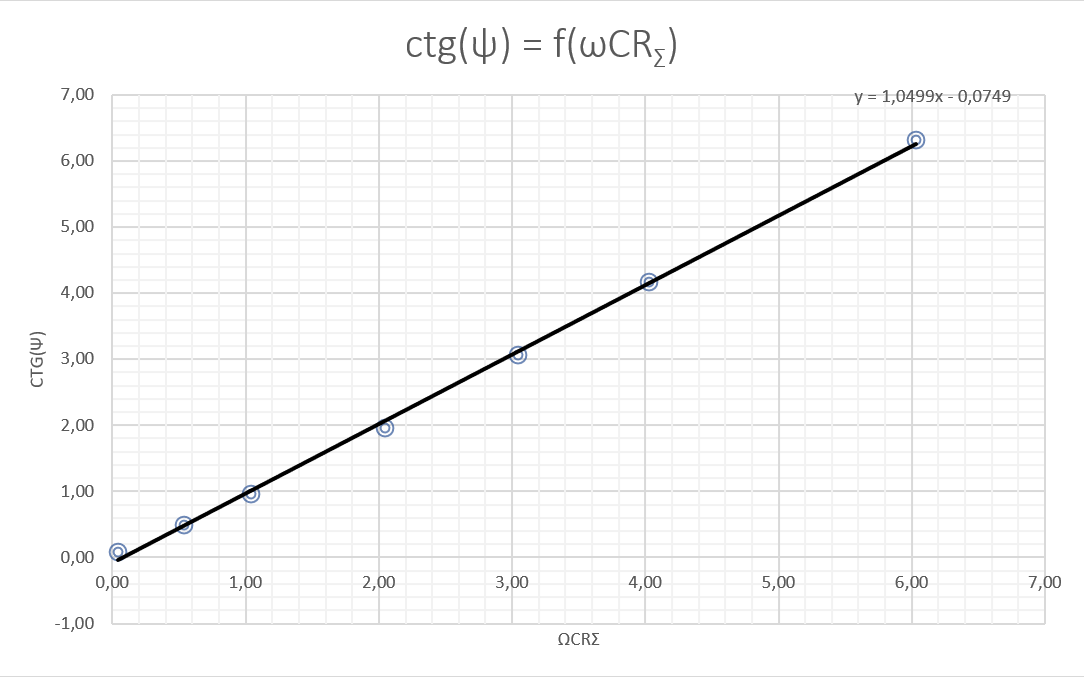
\includegraphics[width=0.95\textwidth]{3.2.1_5.png}\\
\textbf{Рис. 5.} График зависимости котангенса фазового сдвига в цепи от $\omega CR_{\Sigma}$ \\
\end{center}

\hfill \break Уравнение полученной зависимости указано на графике. Теперь рассчитаем теоретически, каким должен быть наклон получившейся прямой. Как известно, полный импеданс $RLC$-цепочки равен:

\begin{equation}\label{ linkname }
Z_{RLC} = R_{\Sigma} + i\omega L + \frac{1}{i\omega C}.
\end{equation}

\hfill \break В соответствии с (5), $\tg{\psi_{I}} = \frac{Im Z}{Re Z} = \frac{\omega L - \frac{1}{\omega C}}{R_{\Sigma}}$, откуда, учитывая, что в нашем случае $L = 0$, получаем:

$$
\ctg(\psi) = \omega R_{\Sigma}C,
$$

\hfill \break то есть исследуемый график зависимости должен представлять прямую с коэффициентом наклона $1$. Как видно из рис. 5, экспериментальное значение коэффициента наклона $-$ 1.05, погрешность равна примерно $12\%$ (систематическая погрешность $+$ погрешность расчета делений $x$ и $x_{0}$ и погрешность определения коэффициента наклона при помощи МНК), следовательно, экспериментальная зависимость отлично сходится с теорией.

\subsection{Исследование сдвига фаз в $RL$-цепи}
\hfill \break В уже собранной согласно рис. 3 схеме закоротим теперь магазин емкостей и установим $\nu = 1$ кГц и $L = 50$ мГн. Тогда реактивное сопротивление: $X_{2} = \omega L = 2\pi \nu L = 314$ Ом. Аналогично предыдущему пункту будем менять сопротивление $R$ от $0$ до $10X_{2}$, фиксируя значение сдвига фаз для каждого значения сопротивления. Результаты занесем в таблицу 3:

\begin{center}
\begin{tabular}{|c|c|c|c|c|c|}\hline
$ R $, Ом & $ x $, дел & $ x_{0} $, дел & $ \psi $, рад & $ R_{\Sigma}/(\omega L) $ & $ ctg(\psi) $\\\hline
0 & 8.50 & 19.00 & 1.41 & 0.14 & 0.17 \\\hline
157 & 6.00 & 19.00 & 0.99 & 0.64 & 0.65 \\\hline
314 & 4.50 & 19.00 & 0.74 & 1.14 & 1.09 \\\hline
628 & 2.50 & 19.00 & 0.41 & 2.14 & 2.28 \\\hline
942 & 2.00 & 19.00 & 0.33 & 3.14 & 2.91 \\\hline
1260 & 1.50 & 19.00 & 0.25 & 4.15 & 3.95 \\\hline
1908 & 1.00 & 19.00 & 0.17 & 6.21 & 5.99 \\\hline
\end{tabular} \\
\hfill \break \textbf {Таблица 3.} Расчеты и измерения для определения разности фаз в $RL$-цепи\\
\end{center}

\hfill \break Построим график зависимости вида $\ctg(\psi) = f(R_{\Sigma}/(\omega L))$, где $R_{\Sigma} = R + R_{L} + r$ $-$ суммарное сопротивление в цепи:

\begin{center}
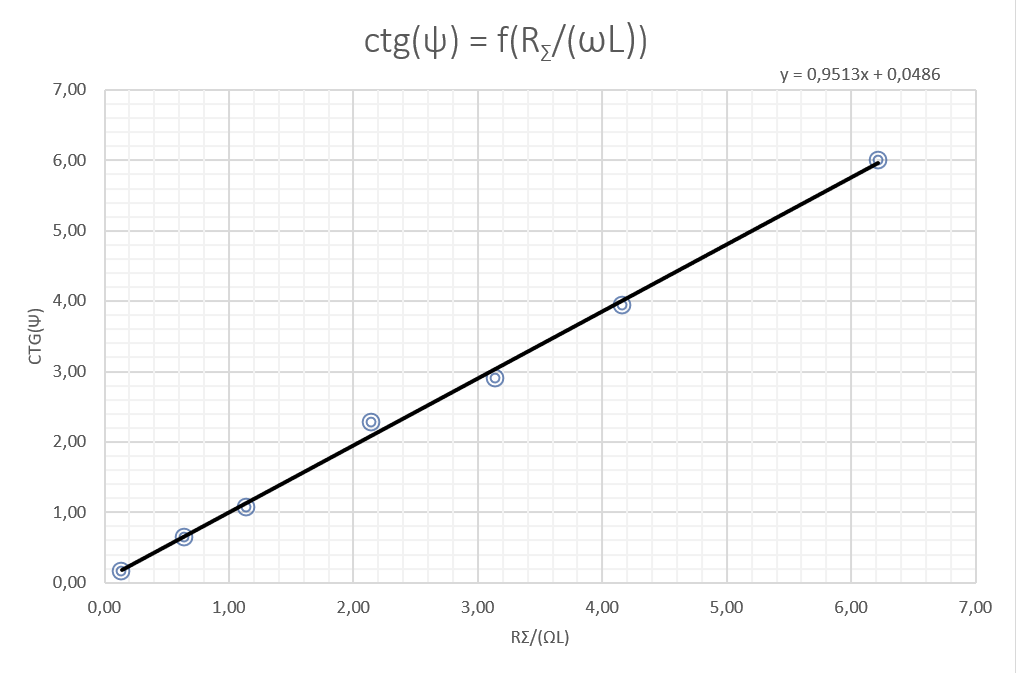
\includegraphics[width=0.95\textwidth]{3.2.1_6.png}\\
\textbf{Рис. 6.} График зависимости котангенса фазового сдвига в цепи от $R_{\Sigma}/(\omega L)$ \\
\end{center}

\hfill \break Как видно из уравнения зависимости, указанного на графике, коэффициент наклона полученной прямой равен приблизительно $0.95$. Проверим это значение при помощи теории. Из уравнений (5) и (10), учитывая, что $C \rightarrow \infty$, получим, что в данном случае:

$$
\ctg(\psi) = \frac{R_{\Sigma}}{\omega L},
$$

\hfill \break что означает, что коэффициент наклона должен быть равен единице, то есть экспериментальное значение почти совпало с рассчитанным теоретически. 

\subsection{Исследование зависимости сдвига фаз от частоты в $RCL$-цепи}
\hfill \break В схеме, уже собранной согласно рис. 3, установим $R = 0, L = 50$ мГн, $C = 0.5$ мкФ. Рассчитаем резонансную частоту при данных параметрах установки: $\nu_{0} = \frac{1}{2\pi \sqrt{LC}} = 1006.6$ Гц, что совпало с экспериментальным наблюдением (при резонансе наблюдается нулевой сдвиг фаз между током и напряжением $-$ формула (5)). Исследуем сдвиг фаз на интервале частот $850 - 1150$ Гц ($|\psi| < \pi/3)$ при $R = 0$ Ом и $R = 100$ Ом. Занесем результаты измерений и расчетов в таблицу 4:

\begin{center}
\begin{tabular}{|c|c|c|c|c|c|}\hline
$ \nu $, Гц & $ x_{0} $, дел & $ x $, дел & $ \nu/\nu_{0} $ & $ \psi $, рад & $ R $, Ом\\\hline
850 & 19.00 & 7.00 & 0.844 & 1.157 & \multirow{11}{*}{0} \\\cline{1 -5}
900 & 17.50 & 5.50 & 0.894 & 0.987 & \multirow{11}{*}{} \\\cline{1 -5}
940 & 17.00 & 4.00 & 0.934 & 0.739 & \multirow{11}{*}{} \\\cline{1 -5}
970 & 16.30 & 2.20 & 0.964 & 0.424 & \multirow{11}{*}{} \\\cline{1 -5}
990 & 16.00 & 1.20 & 0.984 & 0.236 & \multirow{11}{*}{} \\\cline{1 -5}
1000 & 39.00 & 1.10 & 0.993 & 0.089 & \multirow{11}{*}{} \\\cline{1 -5}
1010 & 38.00 & 1.00 & 1.003 & 0.083 & \multirow{11}{*}{} \\\cline{1 -5}
1030 & 37.00 & 4.00 & 1.023 & 0.340 & \multirow{11}{*}{} \\\cline{1 -5}
1060 & 36.50 & 7.00 & 1.053 & 0.602 & \multirow{11}{*}{} \\\cline{1 -5}
1100 & 35.00 & 10.00 & 1.093 & 0.898 & \multirow{11}{*}{} \\\cline{1 -5}
1150 & 33.50 & 11.00 & 1.142 & 1.032 & \multirow{11}{*}{} \\\hline
850 & 19.00 & 3.50 & 0.844 & 0.579 & \multirow{11}{*}{100} \\\cline{1 -5}
900 & 17.50 & 2.50 & 0.894 & 0.449 & \multirow{11}{*}{} \\\cline{1 -5}
940 & 16.70 & 1.30 & 0.934 & 0.245 & \multirow{11}{*}{} \\\cline{1 -5}
970 & 16.00 & 1.00 & 0.964 & 0.196 & \multirow{11}{*}{} \\\cline{1 -5}
990 & 15.70 & 0.50 & 0.984 & 0.100 & \multirow{11}{*}{} \\\cline{1 -5}
1000 & 39.00 & 0.10 & 0.993 & 0.008 & \multirow{11}{*}{} \\\cline{1 -5}
1010 & 38.00 & 0.05 & 1.003 & 0.004 & \multirow{11}{*}{} \\\cline{1 -5}
1030 & 36.00 & 1.50 & 1.023 & 0.131 & \multirow{11}{*}{} \\\cline{1 -5}
1060 & 36.00 & 2.50 & 1.053 & 0.218 & \multirow{11}{*}{} \\\cline{1 -5}
1100 & 35.50 & 4.00 & 1.093 & 0.359 & \multirow{11}{*}{} \\\cline{1 -5}
1150 & 33.00 & 5.50 & 1.142 & 0.524 & \multirow{11}{*}{} \\\hline
\end{tabular} \\
\hfill \break \textbf {Таблица 4.} Расчеты и измерения для определения сдвига фаз в $RLC$-цепи\\
\end{center}

\hfill \break Построим график зависимости сдвига фаз $\psi$ от отношения частот $\nu/\nu_{0}$ при $R = 0$ Ом, где $\psi$ выразим в долях $\pi$. По уровню $\psi$, соответствующему приблизительно $\pi/4$, сможем определить добротность по формуле $Q = \frac{\nu_{0}}{2\Delta\nu}$, где $2\Delta\nu$ $-$ ширина графика при сдвиге фаз $\psi = \pi/4$.

\begin{center}
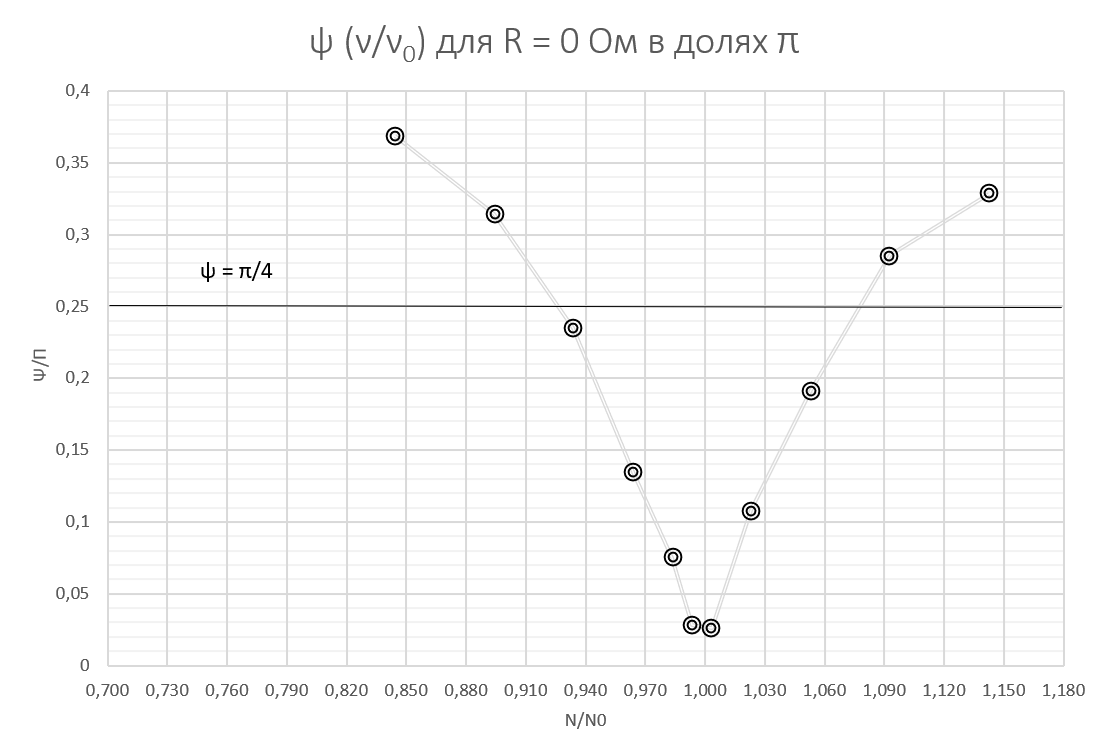
\includegraphics[width=0.95\textwidth]{3.2.1_7.png}\\
\textbf{Рис. 7.} График зависимости фазового сдвига в долях $\pi$ в цепи от отношения текущей частоты к резонансой (при $R = 0$) \\
\end{center}

\hfill \break Как видно из графика, ширина $2\Delta\nu \approx 0.15$, то есть добротность: $Q_{0} = 7.1$. Теоретическое значение добротности при $R = 0$: $Q_{0} = \frac{1}{R_{\Sigma}} \sqrt{\frac{L}{C}} = 7.2$, что неплохо согласуется со значением, полученным экспериментальным путем.

\hfill \break Аналогично построим график зависимости сдвига фаз $\psi$ от отношения частот $\nu/\nu_{0}$ при $R = 100$ Ом, где $\psi$ выразим в долях $\pi$.

\begin{center}
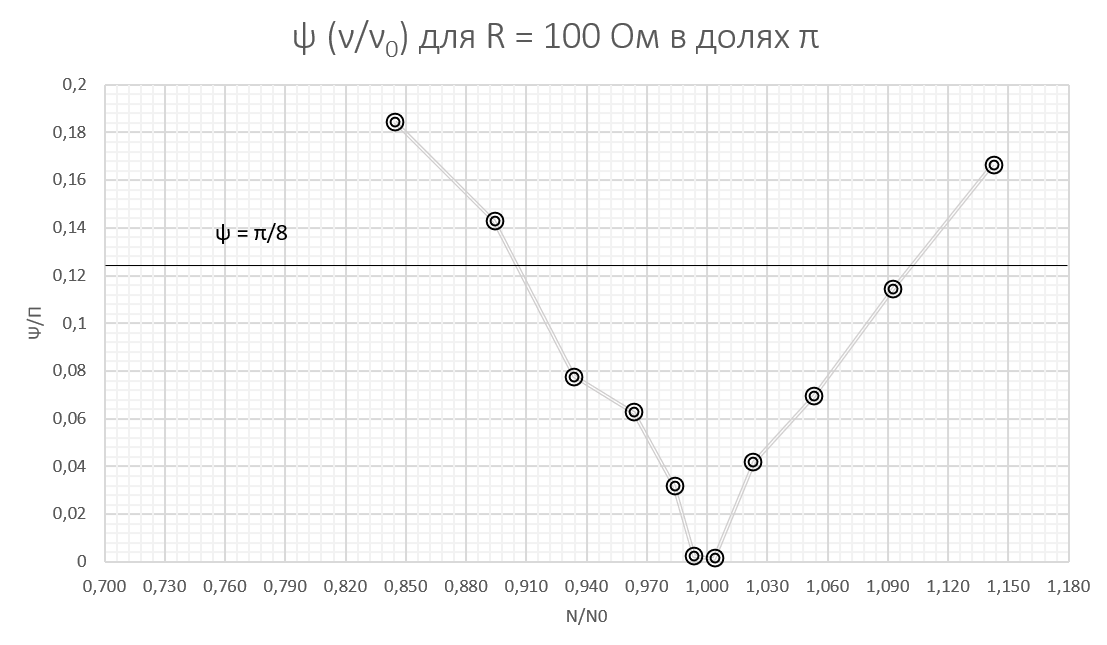
\includegraphics[width=0.95\textwidth]{3.2.1_8.png}\\
\textbf{Рис. 8.} График зависимости фазового сдвига в долях $\pi$ в цепи от отношения текущей частоты к резонансой (при $R = 100$ Ом) \\
\end{center}

\hfill \break Очевидно, из такого графика сложно оценить добротность по уровню $\psi = \pi/4$, поэтому сделаем это при $\psi = \pi/8$.

$$
\tg(\pi/8) = \frac{\omega L - \frac{1}{\omega C}}{R} = Q\frac{(\frac{\omega}{\omega_{0}})^2-1}{\frac{\omega}{\omega_{0}}} = Q\frac{(1+x)^2 - 1}{(1+x)^2} \approx Q \cdot 2x_{\psi = \pi/8}, 
$$

\hfill \break откуда добротность $Q_{100} = 2.1$. Рассчитаем теоретическое значение добротности: $Q_{100} = 2.2$, что снова близко к экспериментальному. Для наглядности занесем полученные значения в таблицу 5:

\begin{center}
\begin{tabular}{|c|c|c|}\hline
$  $ & $ R = 0 $ Ом & $ R = 100 $ Ом \\\hline
$ Q_\text{эксп} $ & 7.1 & 2.1 \\\hline
$ Q_\text{теор} $ & 7.2 & 2.2 \\\hline
\end{tabular} \\
\hfill \break \textbf {Таблица 5.} Теоретические и экспериментальные значения добротности контура для различных значений сопротивления\\
\end{center}

\subsection{Исследование работы фазовращателя}
\hfill \break Соберем схему, изображенную на рис. 4, и установим $C = 0.5$ мкФ, $\nu = 1$ кГц. Подберем сопротивление, при котором сдвиг фаз между входным и выходным напряжениями равен $\pi/2$, $-$ это $R = 1920$ Ом. При этом теоретическое значение $R = \frac{1}{\omega C} = 2$ кОм. Как видно, значения совпадают в пределах погрешности.

\hfill \break Теперь построим векторную диаграмму для фазовращателя:

\begin{center}
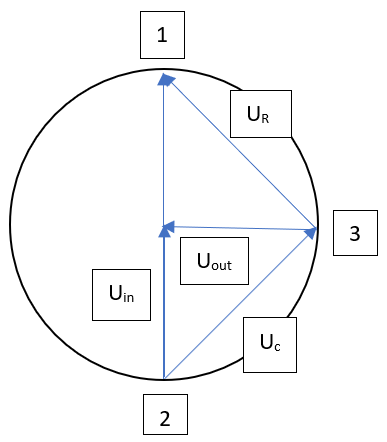
\includegraphics[width=0.45\textwidth]{3.2.1_9.png}\\
\textbf{Рис. 9.} Векторная диаграмма фазовращателя \\
\end{center}

\hfill \break Треугольник (123) равнобедренный и прямоугольный, $\textbf{U}_{in} \perp \textbf{U}_{out}$ $-$ векторы входного и выходного напряжений ортогональны.

\section{Вывод}
\hfill \break В ходе лабораторной работы были изучены зависимости сдвига фаз между током и напряжением от сопротивления в $RC$- ($\ctg(\psi) = \omega R_{\Sigma} C$), $RL$- ($\ctg(\psi) = \frac{R_{\Sigma}}{\omega L}$) и $RLC$-контурах. Для $RLC$-контура были определены значения добротности с резистором $R = 100$ Ом и без него, оба значения оказались близки к рассчитанным теоретически. Также было проведено исследование работы фазовращателя: собрана схема, определено сопротивление, при котором сдвиг фаз между входным и выходным напряжениями равен $\pi/2$ ($R = 1920$ Ом), построена векторная диаграмма. 

\end{document}
